% Options for packages loaded elsewhere
\PassOptionsToPackage{unicode}{hyperref}
\PassOptionsToPackage{hyphens}{url}
%
\documentclass[
]{book}
\usepackage{amsmath,amssymb}
\usepackage{lmodern}
\usepackage{ifxetex,ifluatex}
\ifnum 0\ifxetex 1\fi\ifluatex 1\fi=0 % if pdftex
  \usepackage[T1]{fontenc}
  \usepackage[utf8]{inputenc}
  \usepackage{textcomp} % provide euro and other symbols
\else % if luatex or xetex
  \usepackage{unicode-math}
  \defaultfontfeatures{Scale=MatchLowercase}
  \defaultfontfeatures[\rmfamily]{Ligatures=TeX,Scale=1}
\fi
% Use upquote if available, for straight quotes in verbatim environments
\IfFileExists{upquote.sty}{\usepackage{upquote}}{}
\IfFileExists{microtype.sty}{% use microtype if available
  \usepackage[]{microtype}
  \UseMicrotypeSet[protrusion]{basicmath} % disable protrusion for tt fonts
}{}
\makeatletter
\@ifundefined{KOMAClassName}{% if non-KOMA class
  \IfFileExists{parskip.sty}{%
    \usepackage{parskip}
  }{% else
    \setlength{\parindent}{0pt}
    \setlength{\parskip}{6pt plus 2pt minus 1pt}}
}{% if KOMA class
  \KOMAoptions{parskip=half}}
\makeatother
\usepackage{xcolor}
\IfFileExists{xurl.sty}{\usepackage{xurl}}{} % add URL line breaks if available
\IfFileExists{bookmark.sty}{\usepackage{bookmark}}{\usepackage{hyperref}}
\hypersetup{
  pdftitle={Ráster con R},
  pdfauthor={Danilo A. Verdugo Chaura},
  hidelinks,
  pdfcreator={LaTeX via pandoc}}
\urlstyle{same} % disable monospaced font for URLs
\usepackage{color}
\usepackage{fancyvrb}
\newcommand{\VerbBar}{|}
\newcommand{\VERB}{\Verb[commandchars=\\\{\}]}
\DefineVerbatimEnvironment{Highlighting}{Verbatim}{commandchars=\\\{\}}
% Add ',fontsize=\small' for more characters per line
\usepackage{framed}
\definecolor{shadecolor}{RGB}{248,248,248}
\newenvironment{Shaded}{\begin{snugshade}}{\end{snugshade}}
\newcommand{\AlertTok}[1]{\textcolor[rgb]{0.94,0.16,0.16}{#1}}
\newcommand{\AnnotationTok}[1]{\textcolor[rgb]{0.56,0.35,0.01}{\textbf{\textit{#1}}}}
\newcommand{\AttributeTok}[1]{\textcolor[rgb]{0.77,0.63,0.00}{#1}}
\newcommand{\BaseNTok}[1]{\textcolor[rgb]{0.00,0.00,0.81}{#1}}
\newcommand{\BuiltInTok}[1]{#1}
\newcommand{\CharTok}[1]{\textcolor[rgb]{0.31,0.60,0.02}{#1}}
\newcommand{\CommentTok}[1]{\textcolor[rgb]{0.56,0.35,0.01}{\textit{#1}}}
\newcommand{\CommentVarTok}[1]{\textcolor[rgb]{0.56,0.35,0.01}{\textbf{\textit{#1}}}}
\newcommand{\ConstantTok}[1]{\textcolor[rgb]{0.00,0.00,0.00}{#1}}
\newcommand{\ControlFlowTok}[1]{\textcolor[rgb]{0.13,0.29,0.53}{\textbf{#1}}}
\newcommand{\DataTypeTok}[1]{\textcolor[rgb]{0.13,0.29,0.53}{#1}}
\newcommand{\DecValTok}[1]{\textcolor[rgb]{0.00,0.00,0.81}{#1}}
\newcommand{\DocumentationTok}[1]{\textcolor[rgb]{0.56,0.35,0.01}{\textbf{\textit{#1}}}}
\newcommand{\ErrorTok}[1]{\textcolor[rgb]{0.64,0.00,0.00}{\textbf{#1}}}
\newcommand{\ExtensionTok}[1]{#1}
\newcommand{\FloatTok}[1]{\textcolor[rgb]{0.00,0.00,0.81}{#1}}
\newcommand{\FunctionTok}[1]{\textcolor[rgb]{0.00,0.00,0.00}{#1}}
\newcommand{\ImportTok}[1]{#1}
\newcommand{\InformationTok}[1]{\textcolor[rgb]{0.56,0.35,0.01}{\textbf{\textit{#1}}}}
\newcommand{\KeywordTok}[1]{\textcolor[rgb]{0.13,0.29,0.53}{\textbf{#1}}}
\newcommand{\NormalTok}[1]{#1}
\newcommand{\OperatorTok}[1]{\textcolor[rgb]{0.81,0.36,0.00}{\textbf{#1}}}
\newcommand{\OtherTok}[1]{\textcolor[rgb]{0.56,0.35,0.01}{#1}}
\newcommand{\PreprocessorTok}[1]{\textcolor[rgb]{0.56,0.35,0.01}{\textit{#1}}}
\newcommand{\RegionMarkerTok}[1]{#1}
\newcommand{\SpecialCharTok}[1]{\textcolor[rgb]{0.00,0.00,0.00}{#1}}
\newcommand{\SpecialStringTok}[1]{\textcolor[rgb]{0.31,0.60,0.02}{#1}}
\newcommand{\StringTok}[1]{\textcolor[rgb]{0.31,0.60,0.02}{#1}}
\newcommand{\VariableTok}[1]{\textcolor[rgb]{0.00,0.00,0.00}{#1}}
\newcommand{\VerbatimStringTok}[1]{\textcolor[rgb]{0.31,0.60,0.02}{#1}}
\newcommand{\WarningTok}[1]{\textcolor[rgb]{0.56,0.35,0.01}{\textbf{\textit{#1}}}}
\usepackage{longtable,booktabs,array}
\usepackage{calc} % for calculating minipage widths
% Correct order of tables after \paragraph or \subparagraph
\usepackage{etoolbox}
\makeatletter
\patchcmd\longtable{\par}{\if@noskipsec\mbox{}\fi\par}{}{}
\makeatother
% Allow footnotes in longtable head/foot
\IfFileExists{footnotehyper.sty}{\usepackage{footnotehyper}}{\usepackage{footnote}}
\makesavenoteenv{longtable}
\usepackage{graphicx}
\makeatletter
\def\maxwidth{\ifdim\Gin@nat@width>\linewidth\linewidth\else\Gin@nat@width\fi}
\def\maxheight{\ifdim\Gin@nat@height>\textheight\textheight\else\Gin@nat@height\fi}
\makeatother
% Scale images if necessary, so that they will not overflow the page
% margins by default, and it is still possible to overwrite the defaults
% using explicit options in \includegraphics[width, height, ...]{}
\setkeys{Gin}{width=\maxwidth,height=\maxheight,keepaspectratio}
% Set default figure placement to htbp
\makeatletter
\def\fps@figure{htbp}
\makeatother
\setlength{\emergencystretch}{3em} % prevent overfull lines
\providecommand{\tightlist}{%
  \setlength{\itemsep}{0pt}\setlength{\parskip}{0pt}}
\setcounter{secnumdepth}{5}
\usepackage{booktabs}
\ifluatex
  \usepackage{selnolig}  % disable illegal ligatures
\fi
\usepackage[]{natbib}
\bibliographystyle{plainnat}

\title{Ráster con R}
\author{Danilo A. Verdugo Chaura}
\date{2022-02-08}

\begin{document}
\maketitle

{
\setcounter{tocdepth}{1}
\tableofcontents
}
\hypertarget{part1}{%
\chapter{Plataforma R}\label{part1}}

\hypertarget{hist-orig}{%
\section{Historia y Origen}\label{hist-orig}}

R es un \emph{sistema} o una \emph{plataforma} que surge de un entorno computacional diseñado originalmente para el cálculo estadístico. Nace como un dialecto de \index{S}S el cual es un lenguaje de programación desarrollado por \index{John Chambers}John Chambers (Figura \ref{fig:img-crea-1}) y otros en la antigua ``Bell Telephone Laboratorios'', originalmente miembro de AT \& T Corp.~S se inicia en 1976 como un programa interno de análisis estadístico. En 1988 el sistema fue reescrito desde FORTRAN a C y empezó a parecerse al sistema que tenemos hoy en día (esto fue en la versión 3 del lenguaje S). Lo importante de destacar es el espíritu original por el cual fue diseñado el sistema: facilitar el análisis de datos, primero para ellos y eventualmente, para otros.

\begin{figure}

{\centering 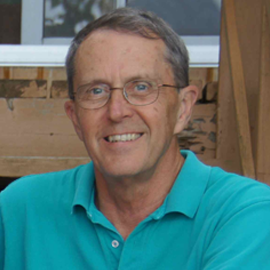
\includegraphics[width=3.75in]{img/john-chambers} 

}

\caption{John Chambers creador de S.}\label{fig:img-crea-1}
\end{figure}

John Chambers describe el anhelo al momento de diseñar el lenguaje S con que ``los usuarios comenzaran en un entorno interactivo, donde no pensaran conscientemente en sí mismos como programadores. Entonces, cuando sus necesidades fuesen más claras y su sofisticación aumentara, deberían ser capaces de transitar gradualmente a la programación, cuando lenguaje y sistema serían más importantes''. La clave fue la transición de usuario a desarrollador. Ellos querían construir un lenguaje que fácilmente podría dar servicio a ambos tipos de usuario. Técnicamente, necesitaban construir un lenguaje que fuese adecuado para el análisis de datos interactivo (basada en línea de comandos), así como para la escritura de programas (como los lenguajes tradicionales de programación).

\begin{figure}

{\centering 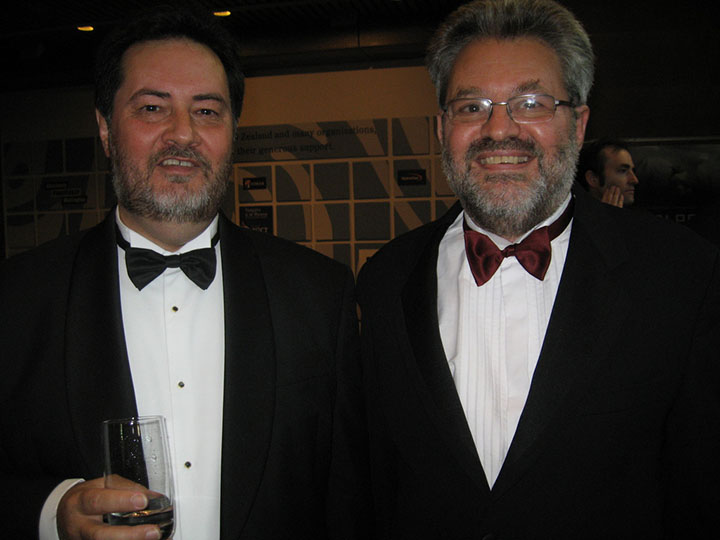
\includegraphics[width=10in]{img/creators} 

}

\caption{Ross Ihaka y Robert Gentleman, los creadores de R.}\label{fig:img-crea}
\end{figure}

En 1991, \index{Ross Ihaka}Ross Ihaka y \index{Robert Gentleman}Robert Gentleman (Figura \ref{fig:img-crea}) en el Departamento de Estadística de la Universidad de Auckland crean R. Inspirado en la filosofía de S pero como un proyecto totalmente abierto. En 1993, se hace público. La experiencia de Robert y Ross sobre el desarrollo de R está documentada en un interesante artículo de 1996 en el Journal of Computational and Graphical Statistics \citep{Ihaka1996}.

Hoy R se ejecuta en casi cualquier sistema operativo o plataforma informática estándar ¡incluso en una playstation 3! Una característica interesante en muchos proyectos de código abierto son las versiones frecuentes. Estos días se produce una liberación anual importante, por lo general en octubre, donde se incorporan nuevas características principales y lanzadas al público. A lo largo del año, se realizarán lanzamientos de corrección de errores en pequeña escala, según sea necesario. Los lanzamientos frecuentes y ciclo de liberación regular indican un permanente y activo desarrollo del software donde se asegura que los errores serán tratados de una manera oportuna. Por supuesto, el árbol principal de código fuente de R se encuentra bajo el control de un pequeño grupo de desarrolladores. Al momento de escribir estas líneas (mayo 2021) nos encontramos en la versión 4.0.5 o \textbf{Shake and Throw}.

Es interesante notar el dato anecdótico que los nombres propios con que se han designado desde la primera versión liberada \emph{Great Pumpkin} (versión 2.14.0, noviembre 2011) o \emph{Trick or Treat} (versión 2.15.2, octubre 2012) entre muchas otras hacen referencia a un capítulo específico de la serie animada \index{Peanuts}\emph{Peanuts} (Figura \ref{fig:img-pea}).

\begin{figure}

{\centering 
\includegraphics[width=7.4in]{img/Peanuts2014} 

}

\caption{Serie animada Peanuts (Snoopy) basada en los comics de Charles Schulz.}\label{fig:img-pea}
\end{figure}

Otra de las ventajas clave que R posee avanzadas capacidades gráficas con \emph{calidad de publicación} cuya existencia se ha asegurado desde el principio del proyecto mediante el control muy fino en todos los aspectos de la composición gráfica.

\hypertarget{dis-plat}{%
\section{Diseño de la Plataforma R}\label{dis-plat}}

El éxito alcanzado por el proyecto R no tiene nada que ver con las herramientas en sí mismas, sino más bien con lo activa que sea la comunidad de usuarios, hoy miles de ellos en todo el mundo se han unido para realizar contribuciones como también ayudar a otros a usar R para todo tipo de nuevas e insospechadas aplicaciones.

El sistema \index{R base}R base o core o núcleo de la plataforma se compone de las herramientas mínimas para su funcionamiento que se encuentra disponible para varios sistemas operativos: Linux, Windows, Mac e incluso su Código Fuente en la denominada \emph{Red Exhaustiva de Archivos R} (\index{Comprehensive R Archive Network}Comprehensive R Archive Network, \index{CRAN}CRAN.

\href{https://cran.r-project.org/}{cran.r-project.org}, es una red de servidores ftp y web en todo el mundo que almacenan versiones idénticas y actualizadas de código y documentación para R)

\hypertarget{rstudio}{%
\section{\texorpdfstring{\index{RStudio}RStudio}{RStudio}}\label{rstudio}}

Aunque R posee un diseño muy avanzado e inteligente a medida que se realizan rutinas para análisis de datos, gráficos, o se generan archivos temporales de esos mismos procesos o se descargan e instalan diversos paquetes de código adicionales se hace muy difícil de mantener y menos aún generar procedimientos claros, organizados y replicables en distintos entornos informáticos, siendo esta última capacidad crítica para la aproximación científica al análisis de datos. RStudio también es una herramienta libre que hace más fácil el trabajo con R, \citet{Loo2012} definen sus principales características como:

\begin{itemize}
\tightlist
\item
  Editor de texto, explorador de archivos, visualizador de gráficos todo en el mismo entorno.
\item
  Trabaja directo con una instalación subyacente de R.
\item
  Organiza el código y mantiene múltiples proyectos.
\item
  Mantiene mi investigación reproducible.
\item
  Mantiene los paquetes en la instalación de R.
\item
  Crea y comparte reportes.
\item
  Comparte el código y colabora con otros usuarios.
\end{itemize}

RStudio hoy es una aplicación y una fundación dedicada al soporte de sus productos de código abierto \footnote{\href{https://www.rstudio.com/}{www.rstudio.com}} como al servicio comercial de capacitación y consultoría en temas estadísticos y R. Su fundador \index{J.J. Allaire}J.J. Allaire también inventa el lenguaje de programación web \emph{ColdFusion}, \emph{Windows Live Writer} (programa para escribir y publicar blog), \emph{FitNow} y \emph{LoseIt} ambas aplicaciones móviles para ejercicio y pérdida de peso entre otros proyectos tecnológicos.

\hypertarget{car-prin}{%
\section{Características Principales}\label{car-prin}}

Algunas propiedades que hacen de RStudio el editor ideal para trabajar con R (tomado de \citet{Loo2012}):\\
\textbf{\emph{Integración con la consola R:}} Escribe comandos directamente en R dentro de RStudio.\\
\textbf{\emph{Ejecución de código:}} Ejecuta código directo desde el editor.\\
\textbf{\emph{Paréntesis inteligente:}} Cierre automático de paréntesis, ilumina selección, cierre de comillas automático. Termina de escribir la palabra previamente iluminada de un menú \index{intellisense}intellisense.\\
\textbf{\emph{Ayuda en línea:}} Acceso directo a la ayuda de lenguaje y sintaxis.\\
\textbf{\emph{Atajos de teclado:}} Tareas repetitivas son asociadas a combinación de teclas. Integra Ayuda, Permite navegar y buscar en las páginas de ayuda nativas de R.\\
\textbf{\emph{Explorador de objetos e Historia:}} Se puede inspeccionar cada objeto creado en la sesión actual de R y su explorador de historia permite recorrer los comandos utilizados desde el actual hasta el primero de la sesión.\\
\textbf{\emph{Navegar por el código:}} Saltar entre funciones, llamadas y reportes, visor de datos y visualización tipo grilla para explorar el contenido de los objetos en la sesión actual.\\
\textbf{\emph{Menús de Importar datos:}} Para los tipos más comunes de archivo, ofrece un sistema de menú que genera el código R necesario. Integración gráfica con zoom, paneo y capacidades de exportación.\\
\textbf{\emph{Gestión de proyectos:}} Facilita el manejo y control de varios proyectos. Control de versión e integra los sistemas de control git y svn.\\
\textbf{\emph{Generación de Documentos:}} Genera pdf, html y otros formatos de reporte usando \index{RMarkdown}RMarkdown, \index{Sweave}Sweave o \index{knitr}knitr.\\
\textbf{\emph{Publicación:}} Publicar reportes y rutinas directo a la web de \emph{\index{Rpubs.com}Rpubs.com.}

\hypertarget{inst-pla}{%
\section{Instalación de Plataforma R y RStudio}\label{inst-pla}}

Primero se debe descargar el paquete de instalación desde el sitio web \href{https://www.r-project.org/}{www.r-project.org} siguiendo el link \textbf{CRAN} y buscar en el listado de servidores espejo el más cercano a la ubicación del usuario. Luego, seleccionar la versión correspondiente al sistema operativo de la máquina a instalar. A continuación, prestar atención y ubicar el link \textbf{install R for the first time} en el apartado \emph{base}.

Finalmente, encontramos el link para la descarga del paquete instalador, siempre será le versión más reciente. Ejecutar el programa y seguir los pasos indicados por el asistente.\footnote{Es importante señalar que el \emph{nombre de usuario} de la sesión Windows donde se realizará la instalación \textbf{no existan} espacios e idealmente no contenga tildes. De ser así, es recomendable crear una nueva sesión con un nombre sin espacios ni tildes.}

Una vez terminada la instalación de R procedemos a instalar el programa RStudio desde el sitio \href{https://www.rstudio.com}{www.rstudio.com} y buscar en la lista de productos \emph{RStudio Desktop.} A continuación, seleccionar la versión \emph{Open Source Edition} que es libre de pago. Finalmente seguir la secuencia de botones correspondiente hasta llegar al punto de descarga del paquete de instalación. Poner especial atención en seleccionar el que corresponda a su versión de sistema operativo. Ejecutar el programa y seguir los pasos indicados por el asistente.

\hypertarget{con-pre}{%
\section{Consideraciones Preliminares}\label{con-pre}}

El entorno de trabajo de RStudio posee una configuración por defecto que presenta una distribución de funcionalidades orientada al uso como entorno interactivo de cálculo y proceso de datos mediante línea de comandos contenido en la ventana \emph{\index{Panel Console}Console} y una vista general de los objetos y variables creadas en la sesión actual en la ventana \index{Panel Environment}\emph{Environment} (Figura \ref{fig:img-gui}).

\begin{figure}

{\centering 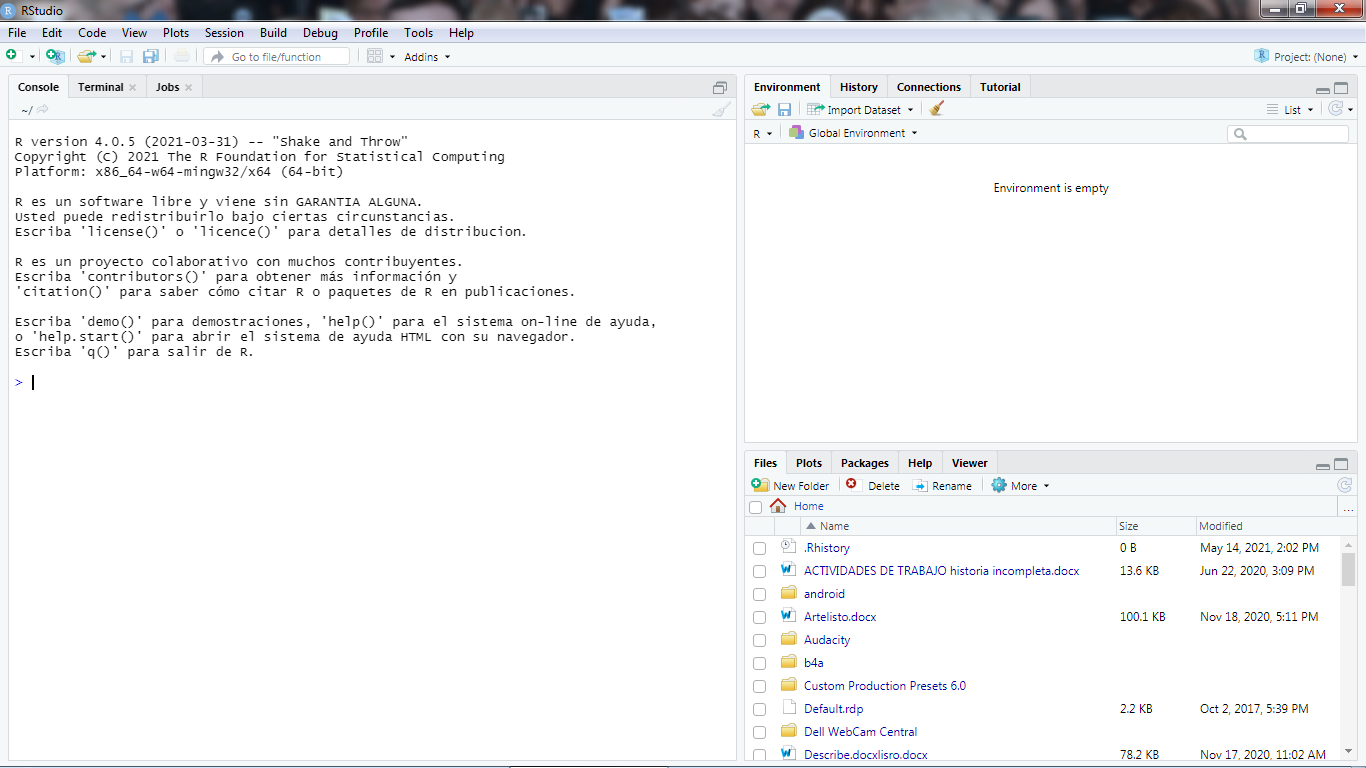
\includegraphics[width=18.97in]{img/GUI} 

}

\caption{Configuración por defecto.}\label{fig:img-gui}
\end{figure}

El tipo de trabajo descrito en el presente texto utiliza metodologías más complejas y extensas que trabajar solo como calculadora o proceso de datos. Por lo tanto, vamos a sugerir una nueva distribución de ventanas que optimicen el trabajo en un tipo de archivos que permiten ir escribiendo largas secuencias de comandos que van desarrollando las tareas de manera secuencial y por seguridad buscamos grabar en disco un archivo que la próxima vez me permita repetir dicha secuencia y continuar o modificar según el caso. Los archivos creados tendrán la extensión \emph{.R} y los denominaremos \emph{\index{scripts}scripts}.

\begin{figure}

{\centering 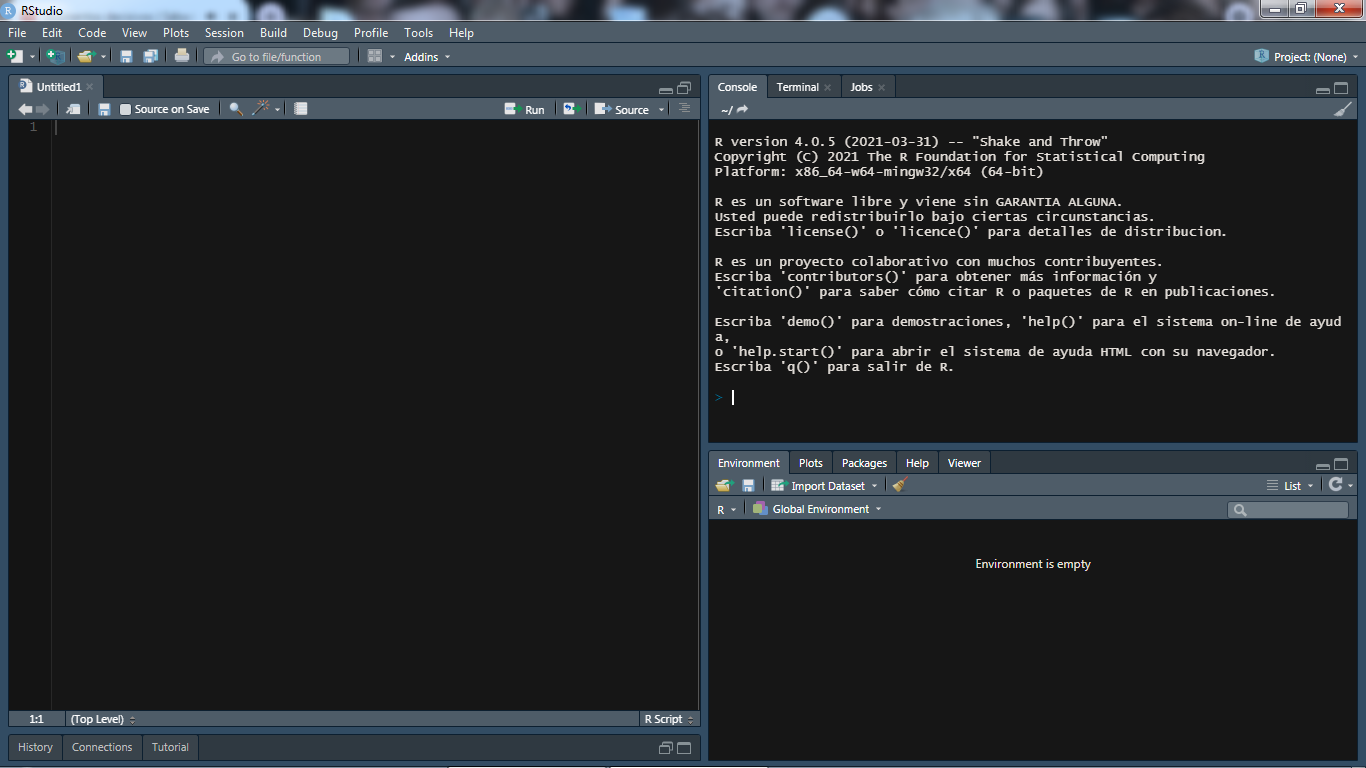
\includegraphics[width=18.97in]{img/gui-final} 

}

\caption{Configuración sugerida.}\label{fig:img-gui-1}
\end{figure}

Una mejor disposición de ventanas es la sugerida en la figura \ref{fig:img-gui-1}. Donde se privilegia el panel izquierdo para extender a altura completa el editor de texto y maximizar el área disponible para escribir y editar scripts y mantiene el panel derecho la consola con su línea de comando.

Otro aspecto importante es el uso de un color de fondo obscuro que reduce la fatiga visual cuando se sienta frente al monitor durante períodos muy prolongados.

Otra característica configurada por defecto es que al momento de salir de una sesión, es guardar el \emph{espacio de trabajo} lo que significa que se crea una imagen de las variables y funciones actuales en un archivo llamado \index{.RData}''.RData''.

Cuando se vuelve a abrir R desde el mismo directorio de trabajo, el espacio de trabajo se cargará y todas estas cosas estarán disponibles. Pero no recomendamos ese comportamiento. Cargar un espacio de trabajo guardado convierte el script cuidadosamente escrito donde todo sucede lógicamente de acuerdo con un plan a algo parecido a un cajón de sastre, lleno de páginas y cuadernos variados que pueden ser o no pertenecientes al trabajo actual.

Para configurar nuestro programa recomendamos cambiar algunos parámetros en la configuración general de la aplicación, para ellos debemos ir a la opción de menú \textbf{\emph{Tools/Global Options}}. (Figura \ref{fig:img-gui-2}).

\begin{figure}

{\centering 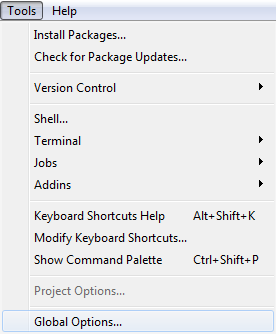
\includegraphics[width=3.83in]{img/mnuOptions} 

}

\caption{Opción de menú para configuración general.}\label{fig:img-gui-2}
\end{figure}

El cuadro de dialogo resume un gran número de parámetros que abarcan detalles del funcionamiento general de RStudio (Figura \ref{fig:img-gui-op-1}).

Los siguientes cambios son necesarios para configurar los aspectos mencionados en punto anterior:

\begin{itemize}
\tightlist
\item
  \emph{General:} Para quitar la carga automática de variables y funciones de la última sesión, debemos en el grupo \textbf{Workspace} quitar el check de \emph{Restore .RData into\ldots{}} y seleccionar la opción \textbf{\emph{Never}} de la lista \emph{Save workspce to .RData\ldots{}} (Figura @ref(fig:img\_gui\_op\_1)).
\end{itemize}

\begin{figure}

{\centering 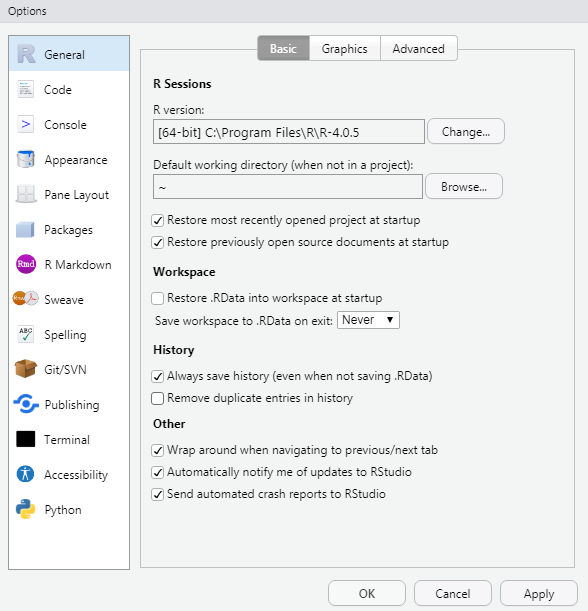
\includegraphics[width=8.17in]{img/ops-general} 

}

\caption{Panel de configuración general.}\label{fig:img-gui-op-1}
\end{figure}

\begin{itemize}
\tightlist
\item
  \emph{Appearance:} La configuración de colores en el editor de texto y los otros cuadros se selecciona en la lista \emph{Editor theme:} y se debe tener especial cuidado en elegir aquel con un fondo negro o muy obscuro (Figura \ref{fig:img-gui-op-2}).
\end{itemize}

\begin{figure}

{\centering 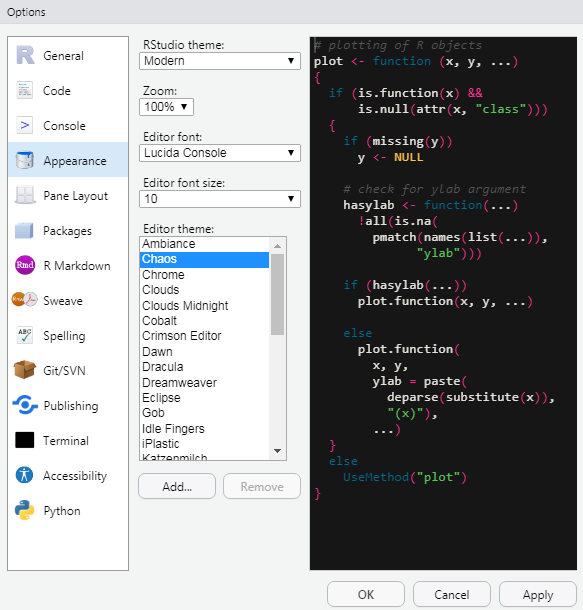
\includegraphics[width=8.1in]{img/ops-app} 

}

\caption{Selección para configuración de colores.}\label{fig:img-gui-op-2}
\end{figure}

\begin{itemize}
\tightlist
\item
  \emph{Pane Layout:} La distribución de los espacios disponibles para optimizar el editor de texto y mantener la línea de comando visible se configura siguiendo las opciones en indicadas en la figura \ref{fig:img-gui-op-3}).
\end{itemize}

\begin{figure}

{\centering 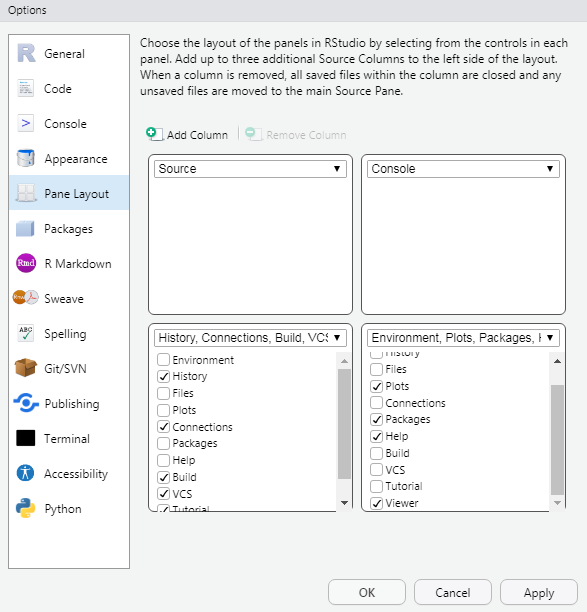
\includegraphics[width=8.15in]{img/ops-panes} 

}

\caption{Configuración de paneles y cuadros.}\label{fig:img-gui-op-3}
\end{figure}

\hypertarget{intro-package}{%
\chapter{\texorpdfstring{\index{paquete}Paquetes}{Paquetes}}\label{intro-package}}

El sistema base, tal como se describe en \ref{dis-plat}, es capaz de ejecutar rutinas y código encapsulado en forma de módulos o paquetes \index{packages}(\emph{packages}) que amplifican y diversifican las posibilidades de cómputo, gráfica, conexiones remotas, generación de documentos y un gran, gran etc.

\begin{quote}
El \textbf{sistema base o core} también se forma de un conjunto de paquetes.
\end{quote}

Además de las funciones más fundamentales el sistema base incluye los paquetes
\index{paquete!utils}utils, \index{paquete!stats}stats, \index{paquete!datasets}datasets, \index{paquete!graphics}graphics, \index{paquete!grDevices}grDevices, \index{paquete!grid}grid, \index{paquete!methods}methods, \index{paquete!tools}tools, \index{paquete!parallel}parallel, \index{paquete!compiler}compiler, \index{paquete!splines}splines, \index{paquete!tcltk}tcltk, \index{paquete!stats4}stats4 y algunos paquetes \emph{recomendados}: \index{paquete!boot}boot, \index{paquete!class}class, \index{paquete!cluster}cluster, \index{paquete!codetools}codetools, \index{paquete!foreign}foreign, \index{paquete!KernSmooth}KernSmooth, \index{paquete!lattice}lattice, \index{paquete!mgcv}mgcv, \index{paquete!nlme}nlme, \index{paquete!rpart}rpart, \index{paquete!survival}survival, \index{paquete!MASS}MASS, \index{paquete!spatial}spatial, \index{paquete!nnet}nnet, \index{paquete!Matrix}Matrix.

Cuando se descarga una instalación nueva de R desde CRAN, se obtiene todos los paquetes mencionados, que representa un gran porcentaje de la funcionalidad del sistema.

\hypertarget{pack-search}{%
\section{Búsqueda}\label{pack-search}}

Además de la gran cantidad de paquetes instalados por defecto, existe una gran cantidad de paquetes opcionales disponibles.

\begin{itemize}
\tightlist
\item
  A noviembre 2021 existen 18.407 paquetes en CRAN que han sido desarrollados por los usuarios y programadores alrededor del mundo cada uno de ellos diseñado para un campo en especial.
\item
  También hay muchos paquetes asociados con el proyecto \index{Bioconductor}\textbf{Bioconductor}\footnote{\href{https://www.bioconductor.org/}{www.bioconductor.org}}, (detalles en \ref{bioconductor}).
\item
  Las personas a menudo hacen sus propios paquetes y los hacen disponibles en sus sitios web personales; en realidad no hay manera confiable de realizar un seguimiento de cuántos paquetes están disponibles de este modo.
\item
  Hay una serie de paquetes que se desarrollan en los repositorios de GitHub y BitBucket pero no existe ninguna lista fiable de todos estos paquetes.
\end{itemize}

El mejor método para buscar en la web, nuevos paquetes es utilizar el sitio \href{https://rseek.org/}{rseek.org} (Figura \ref{fig:img-pack-3}) usando palabras claves y potenciado por el motor de búsqueda de Google.

\begin{figure}

{\centering 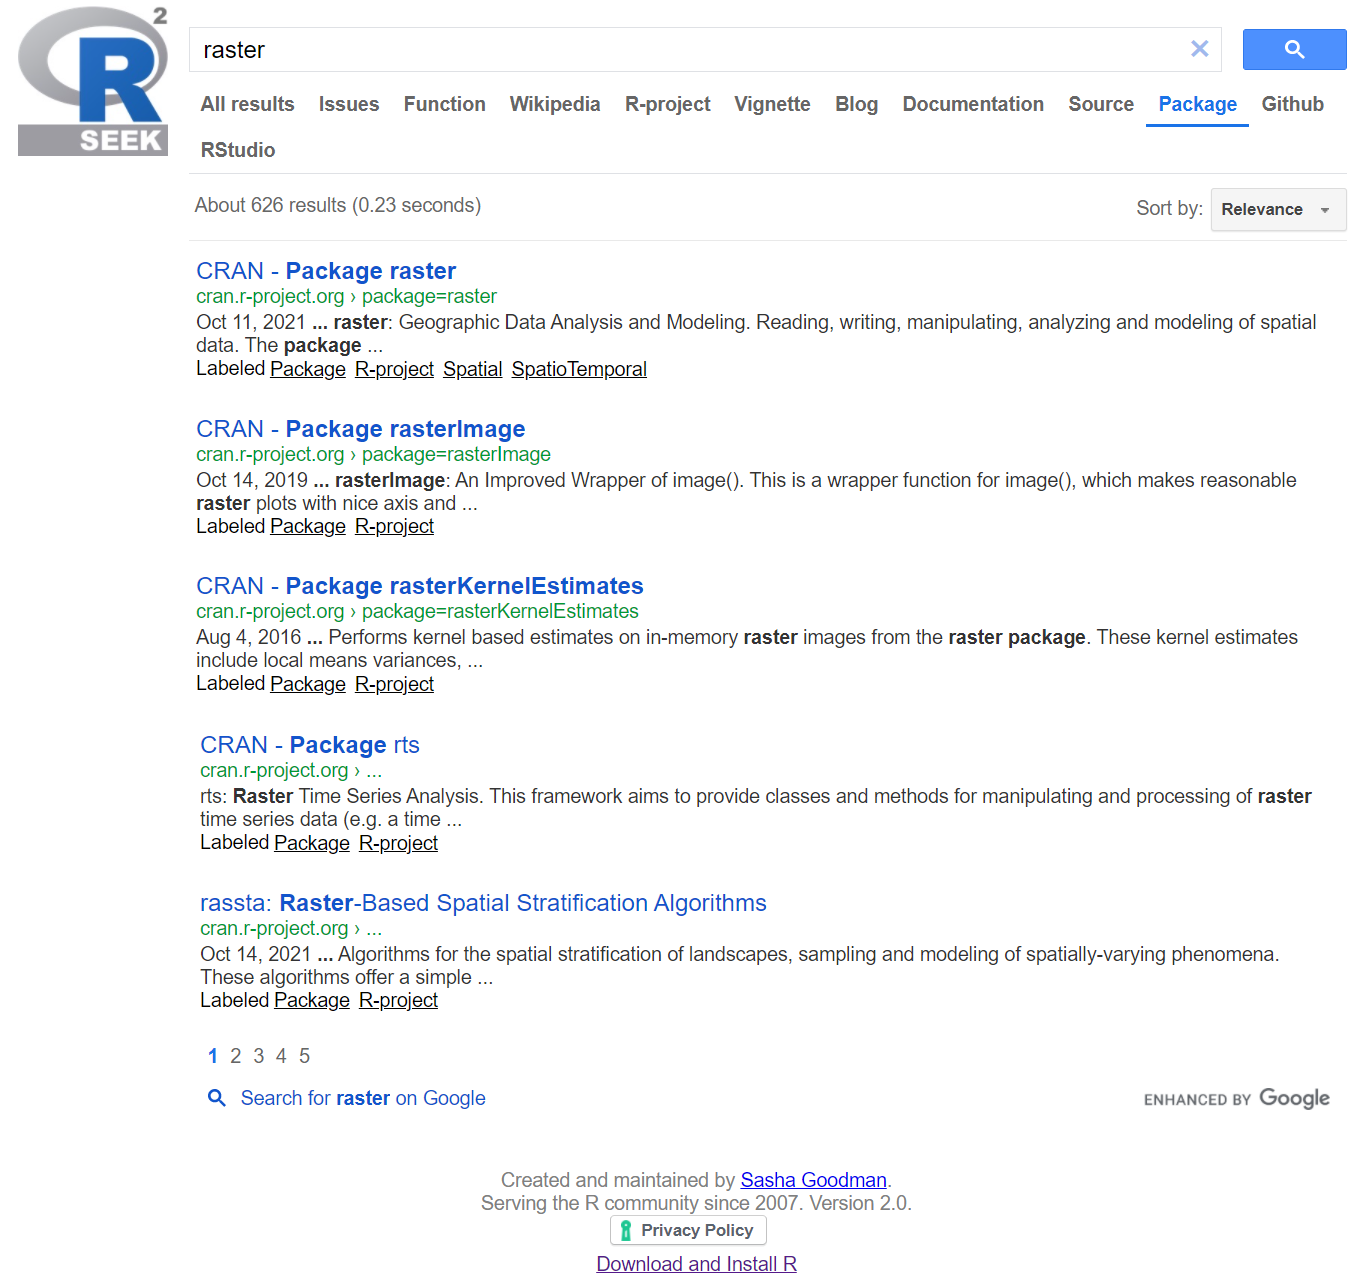
\includegraphics[width=18.96in]{img/pack3} 

}

\caption{Sitio web de búsqueda de contenido asociado a R, modo 'Package'.}\label{fig:img-pack-3}
\end{figure}

Generalmente los resultados siempre serán múltiples y variados.

\hypertarget{pack-install}{%
\section{Instalación}\label{pack-install}}

Una vez identificado un paquete que ofrece las funcionalidades deseadas se debe instalar en nuestro ambiente R y dejarlo disponible para cuando se necesite. El entorno RStudio cuenta con un panel específico (Figura \ref{fig:img-pack-1}).

\begin{figure}

{\centering 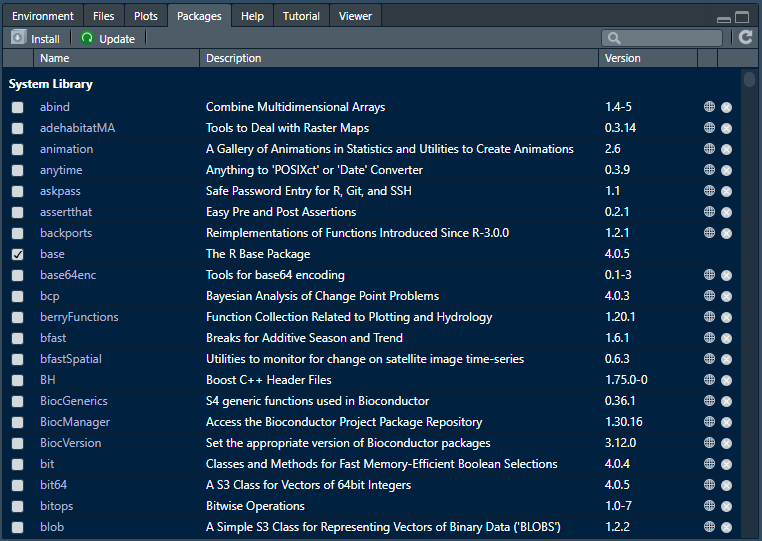
\includegraphics[width=10.58in]{img/pack1} 

}

\caption{Panel Packages.}\label{fig:img-pack-1}
\end{figure}

Que junto al listado de paquetes ya instalados se dispone de opciones para instalar 
\includegraphics[width=0.46875in,height=\textheight]{img/pack4.png} y actualizar 
\includegraphics[width=0.52083in,height=\textheight]{img/pack5.png} (\ref{pack-update}) los existentes.

\hypertarget{pack-cuadro}{%
\subsection{Cuadro Diálogo}\label{pack-cuadro}}

El botón \textbf{Install} levanta un cuadro de diálogo con las opciones de configuración (Figura \ref{fig:img-pack-4}) para instalar paquetes disponibles en CRAN o los paquetes descargados en formato \emph{.zip} de sitios no oficiales.

\begin{figure}

{\centering 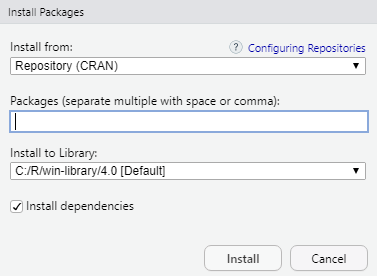
\includegraphics[width=5.24in]{img/pack2} 

}

\caption{Opciones de Instalación vía RStudio.}\label{fig:img-pack-4}
\end{figure}

\hypertarget{pack-install-code}{%
\subsection{\texorpdfstring{Función \emph{install.packages()}}{Función install.packages()}}\label{pack-install-code}}

Un segundo método de instalación es utilizar la función R escrita directamente en la consola y reemplazando \emph{nombre} por el paquete deseado.

\index{install.packages()}

\begin{Shaded}
\begin{Highlighting}[]
\FunctionTok{install.packages}\NormalTok{(}\StringTok{"nombre"}\NormalTok{)}
\end{Highlighting}
\end{Shaded}

\hypertarget{pack-update}{%
\section{Actualización}\label{pack-update}}

El botón 
\includegraphics[width=0.52083in,height=\textheight]{img/pack5.png} del panel paquetes levanta el cuadro de diálogo diseñado para la selección de los paquetes a actualizar. La lista solo muestra aquellos disponibles de actualización (Figura \ref{fig:img-pack-5}).

\begin{figure}

{\centering 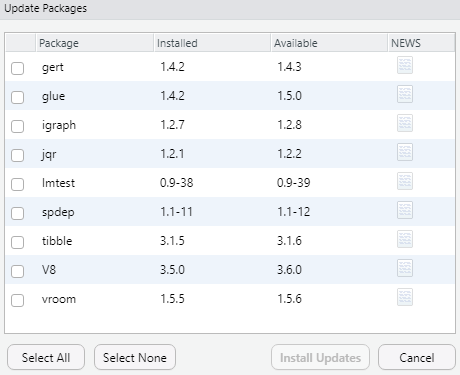
\includegraphics[width=6.39in]{img/pack6} 

}

\caption{Opciones de Instalación vía RStudio.}\label{fig:img-pack-5}
\end{figure}

\hypertarget{sin-bas}{%
\chapter{Sintaxis Básica de R}\label{sin-bas}}

\hypertarget{op-num}{%
\section{Operaciones Numéricas}\label{op-num}}

De acuerdo con la configuración de ventanas descrita en el punto anterior la ventana \emph{Console} se encuentra en la esquina superior derecha junto a las ventanas \index{Terminal}\emph{Terminal} y \index{Jobs}\emph{Jobs}. En ella trabajaremos interactivamente mediante la línea de comando, su uso puede ser comparado con el uso de una calculadora electrónica que siempre está a la espera del ingreso de una instrucción a continuación del símbolo \textbf{\textgreater{}}.

La dinámica de uso es ir ingresando el texto que define la operación o instrucción a realizar y finalizar con la tecla \textbf{Intro}:

\begin{Shaded}
\begin{Highlighting}[]
\DecValTok{1} \SpecialCharTok{+} \DecValTok{2} \SpecialCharTok{+} \DecValTok{3}
\end{Highlighting}
\end{Shaded}

Y R responde con la evaluación inmediata de la operación:

\begin{verbatim}
## [1] 6
\end{verbatim}

Los espacios en blanco son removidos automáticamente y la orden es evaluada normalmente:

\begin{Shaded}
\begin{Highlighting}[]
\DecValTok{1}\SpecialCharTok{+}\DecValTok{2}         \SpecialCharTok{+}       \DecValTok{3}
\end{Highlighting}
\end{Shaded}

\begin{verbatim}
## [1] 6
\end{verbatim}

Cuando la instrucción se extiende por más de una línea, R se encarga de interpretar la estructura y completitud para ser evaluada:

\begin{Shaded}
\begin{Highlighting}[]
\DecValTok{12} \SpecialCharTok{+} \DecValTok{3} \SpecialCharTok{{-}} 
  \DecValTok{5} \SpecialCharTok{+} 
  \DecValTok{5}
\end{Highlighting}
\end{Shaded}

\begin{verbatim}
## [1] 15
\end{verbatim}

También puedes usar el símbolo `punto y coma' (\emph{;}) para separar secuencias de instrucciones, pero escritas en la misma línea de código.

El editor ofrece algunas facilidades al usuario como el \emph{historial de órdenes} de las instrucciones digitadas en orden reverso para evitar el retipeo de una instrucción muy extensa. Recorrer con las flechas verticales hasta encontrar el texto buscado y solo editar los cambios requeridos. También cuenta con un potente \emph{motor de finalización inteligente} que permite obtener ayuda a medida que se escribe nombre de funciones o comandos y cuando se trabaja con scripts también nombres de funciones o variables. Por último, para limpiar todo el texto escrito presionar la tecla \emph{escape}.

Se pueden utilizar los símbolos aritméticos tradicionales +, -, *, / y \(^\wedge\) \footnote{El acento circunflejo \(^\wedge\) se utiliza para la potenciación (se obtiene combinando las teclas alt+94) también se puede reemplazar con \(**\). Además, existe la \emph{operación módulo} (\%\%) y la \emph{división entera} (\%/\%).}. Además se encuentran disponibles las funciones \emph{log}, \emph{exp}, \emph{sin}, \emph{cos}, \emph{tan}, \emph{sqrt} entre muchas otras bien conocidas. También existe el valor de \emph{pi}.

\begin{Shaded}
\begin{Highlighting}[]
\DecValTok{1} \SpecialCharTok{+} \DecValTok{2} \SpecialCharTok{{-}} \DecValTok{3} \SpecialCharTok{*} \DecValTok{4} \SpecialCharTok{/} \DecValTok{5}\SpecialCharTok{**}\DecValTok{6}\NormalTok{; }\FunctionTok{sin}\NormalTok{(}\FloatTok{0.33}\NormalTok{); }\FunctionTok{acos}\NormalTok{(}\FloatTok{0.253}\NormalTok{) ; }\FunctionTok{sqrt}\NormalTok{(}\DecValTok{4}\NormalTok{)}
\end{Highlighting}
\end{Shaded}

\begin{verbatim}
## [1] 2.999232
\end{verbatim}

\begin{verbatim}
## [1] 0.324043
\end{verbatim}

\begin{verbatim}
## [1] 1.315016
\end{verbatim}

\begin{verbatim}
## [1] 2
\end{verbatim}

\begin{Shaded}
\begin{Highlighting}[]
\DecValTok{9} \SpecialCharTok{\%\%} \DecValTok{4}
\end{Highlighting}
\end{Shaded}

\begin{verbatim}
## [1] 1
\end{verbatim}

\begin{Shaded}
\begin{Highlighting}[]
\FloatTok{13.5} \SpecialCharTok{\%/\%} \DecValTok{2}
\end{Highlighting}
\end{Shaded}

\begin{verbatim}
## [1] 6
\end{verbatim}

\begin{Shaded}
\begin{Highlighting}[]
\NormalTok{pi}
\end{Highlighting}
\end{Shaded}

\begin{verbatim}
## [1] 3.141593
\end{verbatim}

También se debe tener en cuenta que los números muy grandes o pequeños serán automáticamente convertidos a notación científica.

\begin{Shaded}
\begin{Highlighting}[]
\DecValTok{1}\SpecialCharTok{/}\DecValTok{100000000000000000}
\end{Highlighting}
\end{Shaded}

\begin{verbatim}
## [1] 1e-17
\end{verbatim}

\begin{Shaded}
\begin{Highlighting}[]
\DecValTok{1}\SpecialCharTok{*}\DecValTok{100000000000000000}
\end{Highlighting}
\end{Shaded}

\begin{verbatim}
## [1] 1e+17
\end{verbatim}

En operaciones más complejas se recomienda el uso de \emph{()} para fijar el orden o \emph{precedencia} de las operaciones. Se acepta \emph{anidar} los paréntesis (()).

\begin{Shaded}
\begin{Highlighting}[]
\DecValTok{3} \SpecialCharTok{*} \DecValTok{5} \SpecialCharTok{+} \DecValTok{1}
\end{Highlighting}
\end{Shaded}

\begin{verbatim}
## [1] 16
\end{verbatim}

\begin{Shaded}
\begin{Highlighting}[]
\DecValTok{3} \SpecialCharTok{*}\NormalTok{ (}\DecValTok{5} \SpecialCharTok{+} \DecValTok{1}\NormalTok{)}
\end{Highlighting}
\end{Shaded}

\begin{verbatim}
## [1] 18
\end{verbatim}

\begin{Shaded}
\begin{Highlighting}[]
\DecValTok{1} \SpecialCharTok{+}\NormalTok{ (}\DecValTok{3} \SpecialCharTok{+}\NormalTok{ (}\DecValTok{1} \SpecialCharTok{+} \DecValTok{2}\NormalTok{) }\SpecialCharTok{/} \DecValTok{3}\NormalTok{)}
\end{Highlighting}
\end{Shaded}

\begin{verbatim}
## [1] 5
\end{verbatim}

Las operaciones lógicas se realizan utilizando ciertos símbolos o combinaciones de ellos para obtener resultados lógicos:

\begin{Shaded}
\begin{Highlighting}[]
\DecValTok{2} \SpecialCharTok{==} \DecValTok{3}
\end{Highlighting}
\end{Shaded}

\begin{verbatim}
## [1] FALSE
\end{verbatim}

\begin{Shaded}
\begin{Highlighting}[]
\DecValTok{2} \SpecialCharTok{\textless{}} \DecValTok{3}
\end{Highlighting}
\end{Shaded}

\begin{verbatim}
## [1] TRUE
\end{verbatim}

Revisa cuadro \ref{tab:tabla_31_1} para una lista completa de los caracteres y su significado en las operaciones lógicas.

Otros componentes del lenguaje R son: valor lógico verdadero \emph{TRUE} y falso \emph{FALSE}, infinitud positiva \textbf{Inf} y negativa \textbf{-Inf}, no disponible \textbf{NA}, no es un número \textbf{NaN} y nulo o vacío \textbf{NULL}.

Finalmente, no podemos intercambiar mayúsculas o minúsculas al momento de escribir los nombres de instrucciones (por ej. \emph{sin} no es igual a \emph{Sin}). Y en R todo es un \emph{objeto} que pertenecen a cierto tipo de \emph{clases}. Así cada uno de ellos tendrá comportamientos y usos diferentes.

\begin{Shaded}
\begin{Highlighting}[]
\FunctionTok{class}\NormalTok{(}\DecValTok{1}\NormalTok{)}
\end{Highlighting}
\end{Shaded}

\begin{verbatim}
## [1] "numeric"
\end{verbatim}

\begin{Shaded}
\begin{Highlighting}[]
\FunctionTok{class}\NormalTok{(}\StringTok{"palabra"}\NormalTok{)}
\end{Highlighting}
\end{Shaded}

\begin{verbatim}
## [1] "character"
\end{verbatim}

\begin{Shaded}
\begin{Highlighting}[]
\FunctionTok{class}\NormalTok{(sqrt)}
\end{Highlighting}
\end{Shaded}

\begin{verbatim}
## [1] "function"
\end{verbatim}

\begin{Shaded}
\begin{Highlighting}[]
\FunctionTok{class}\NormalTok{(}\DecValTok{1} \SpecialCharTok{!=} \DecValTok{1}\NormalTok{)}
\end{Highlighting}
\end{Shaded}

\begin{verbatim}
## [1] "logical"
\end{verbatim}

\begin{Shaded}
\begin{Highlighting}[]
\FunctionTok{class}\NormalTok{(}\ConstantTok{TRUE}\NormalTok{)}
\end{Highlighting}
\end{Shaded}

\begin{verbatim}
## [1] "logical"
\end{verbatim}

\begin{Shaded}
\begin{Highlighting}[]
\FunctionTok{class}\NormalTok{(}\FunctionTok{Sys.Date}\NormalTok{())}
\end{Highlighting}
\end{Shaded}

\begin{verbatim}
## [1] "Date"
\end{verbatim}

\hypertarget{asig}{%
\section{Asignación}\label{asig}}

El proceso de almacenar cualquiera de los objetos ya descritos, o el resultado de las operaciones en memoria RAM y hacerlo persistente a lo largo de la sesión actual de trabajo se denomina \index{asignación}\emph{asignación}. Resultados intermedios se deben ir asignado con un nombre fácilmente identificable y memorizables.\footnote{Los nombres de los objetos deben en lo posible \emph{resumir} el contenido, evitar nombres \emph{genéricos} como \emph{a} u \emph{X} y no ambiguos como \emph{variable} o \emph{constante}. Pueden contener letras, números, puntos y guiones o \emph{barra baja} (\_). Siempre debe comenzar con una letra o punto.}

Es conveniente adoptar un estilo de escritura para los nombres de los objetos y para ellos existen varios métodos entre los cuales podemos destacar:

\begin{itemize}
\tightlist
\item
  \textbf{\emph{lowercase:}} todominusculas.
\item
  \textbf{\emph{UPPERCASE:}} TODOMAYUSCULAS.
\item
  \textbf{\emph{UpperCamelCase:}} PrimeraMayusculaSiguientesBajas.
\item
  \textbf{\emph{lowerCamelCase:}} primeraMinusculaSiguientesMayusculas.
\item
  \textbf{\emph{period.separated:}} separada.por.punto.
\item
  \textbf{\emph{snake\_case:}} separada\_por\_guion\_bajo.
\end{itemize}

En el sitio web \href{https://style.tidyverse.org/}{style.tidyverse.org} donde se discuten buenas prácticas para el uso de R se recomienda el último tipo.

La forma de realizar una asignación tiene la forma general:

\begin{equation} \label{eq:solve}
nombre = valor
\end{equation}

Donde \(nombre\) es el identificador o nombre del objeto o variable que se busca crear y almacenar en memoria, \(=\) el operador de asignación (no confundir con \emph{==}) y \(valor\) es el contenido a almacenar.\footnote{En R se ha utilizado tradicionalmente como operador de asignación \textbf{\textless-} que viene desde la primera versión de R, dado que su origen proviene del lenguaje \textbf{S} y a la vez éste fue inspirado por el lenguaje \index{APL}\emph{APL} (A Programming Language, \index{Kenneth Iverson}\emph{Kenneth Iverson en 1957-62}) que utilizaba dicho carácter ya que el símbolo \emph{=} se utilizaba solo para prueba de igualdad.}

\begin{Shaded}
\begin{Highlighting}[]
\NormalTok{radio\_estimado }\OtherTok{=} \FloatTok{135.45}
\end{Highlighting}
\end{Shaded}

\(nombre\) será sintácticamente válido cuando consta de letras, números o punto y comienza con \textbf{una letra o el punto}, pero \emph{no seguido de un número}. Los nombres como ``.2var'' no son válidos, ni tampoco las palabras reservadas.

En la actualidad el uso \index{<-}\textless- o = es casi indistinto, pero en casos muy específicos (y técnicos) existen diferencias. En nuestro libro recomendamos el uso de \textless- ya que es un poco más cómodo de tipear que el carácter =.

\begin{Shaded}
\begin{Highlighting}[]
\NormalTok{variable }\OtherTok{\textless{}{-}}\NormalTok{ (}\FloatTok{112.33} \SpecialCharTok{{-}} \DecValTok{45}\NormalTok{) }\SpecialCharTok{/} \DecValTok{105}
\end{Highlighting}
\end{Shaded}

Una vez escrita la asignación y presionado \emph{intro} se realiza la operación, se crea el objeto en memoria con nombre \emph{variable} y la línea de comando se limpia. Para conocer el resultado de la operación podemos:

\begin{figure}

{\centering 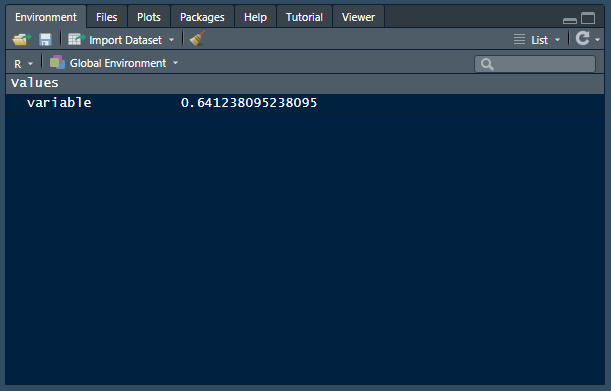
\includegraphics[width=8.49in]{img/enviroment} 

}

\caption{Panel Environment.}\label{fig:img-lan-1}
\end{figure}

\begin{enumerate}
\def\labelenumi{\arabic{enumi}.}
\item
  Buscar el resultado en el panel \textbf{\emph{Environment}} en la esquina inferior derecha (Figura \ref{fig:img-lan-1}).
\item
  Escribir la asignación dentro de un juego de paréntesis redondos \textbf{()} que obliga imprimir el resultado de la evaluación de la expresión.
\end{enumerate}

\begin{Shaded}
\begin{Highlighting}[]
\NormalTok{(variable }\OtherTok{\textless{}{-}}\NormalTok{ (}\FloatTok{112.33} \SpecialCharTok{{-}} \DecValTok{45}\NormalTok{) }\SpecialCharTok{/} \DecValTok{105}\NormalTok{)}
\end{Highlighting}
\end{Shaded}

\begin{verbatim}
## [1] 0.6412381
\end{verbatim}

\begin{enumerate}
\def\labelenumi{\arabic{enumi}.}
\setcounter{enumi}{2}
\tightlist
\item
  Volver a escribir el nombre y presionar intro.
\end{enumerate}

\begin{Shaded}
\begin{Highlighting}[]
\NormalTok{variable}
\end{Highlighting}
\end{Shaded}

\begin{verbatim}
## [1] 0.6412381
\end{verbatim}

\begin{enumerate}
\def\labelenumi{\arabic{enumi}.}
\setcounter{enumi}{3}
\tightlist
\item
  Utilizar el comando \index{print()}\emph{print()}.
\end{enumerate}

\begin{Shaded}
\begin{Highlighting}[]
\FunctionTok{print}\NormalTok{(variable)}
\end{Highlighting}
\end{Shaded}

\begin{verbatim}
## [1] 0.6412381
\end{verbatim}

El principal objetivo de almacenar en memoria es la reutilización de dichos contenidos:

\begin{Shaded}
\begin{Highlighting}[]
\NormalTok{radio\_inicial }\OtherTok{\textless{}{-}} \FloatTok{15.43} \SpecialCharTok{+} \FloatTok{36.315} \SpecialCharTok{*}\NormalTok{ (}\DecValTok{3} \SpecialCharTok{*} \DecValTok{5}\NormalTok{)}
\NormalTok{(area\_base }\OtherTok{\textless{}{-}}\NormalTok{ pi }\SpecialCharTok{*}\NormalTok{ radio\_inicial }\SpecialCharTok{**} \DecValTok{2}\NormalTok{)}
\end{Highlighting}
\end{Shaded}

\begin{verbatim}
## [1] 985748.9
\end{verbatim}

Al asignar un nuevo contenido con el mismo nombre, el anterior se elimina de memoria y se crea un nuevo objeto.

\begin{Shaded}
\begin{Highlighting}[]
\NormalTok{x }\OtherTok{\textless{}{-}} \DecValTok{5}
\NormalTok{x }\OtherTok{\textless{}{-}} \StringTok{"hola"}
\NormalTok{x}
\end{Highlighting}
\end{Shaded}

\begin{verbatim}
## [1] "hola"
\end{verbatim}

El comando \index{ls()}\texttt{ls()} me permite listar todos los objetos almacenados en mi sesión actual y \index{rm()}\texttt{rm(list\ =\ ls())} borrará la totalidad de objetos de mi sesión actual.

\hypertarget{nat-vec}{%
\section{Naturaleza Vectorial}\label{nat-vec}}

En todas las ocasiones que hemos escrito una operación aritmética o impreso un resultado R crea automáticamente un \index{vector}\emph{vector}\footnote{Un \textbf{\emph{Vector}} es el tipo de objeto más básico del lenguaje R. Un \emph{vector} puede contener cero o más objetos, y siempre serán de la misma clase.} con una longitud que corresponde a los valores por almacenar.

Si estudiamos el ejemplo siguiente:

\begin{Shaded}
\begin{Highlighting}[]
\DecValTok{5}
\end{Highlighting}
\end{Shaded}

\begin{verbatim}
## [1] 5
\end{verbatim}

\begin{Shaded}
\begin{Highlighting}[]
\FunctionTok{ls}\NormalTok{()}
\end{Highlighting}
\end{Shaded}

\begin{verbatim}
## [1] "area_base"     "radio_inicial" "variable"      "x"
\end{verbatim}

Vemos un \textbf{{[}1{]}} antecediendo al número 5 que indica que se trata del primer (y único en este caso) elemento, mientras que en el caso del comando \emph{ls()} la lista de respuesta por cada renglón que se extienda en la consola antecederá su correspondiente {[}{]} señalando la posición en el vector generado automáticamente.

\hypertarget{fun-c}{%
\subsection{\texorpdfstring{Función \textbf{\texttt{c()}} para crear vectores}{Función c() para crear vectores}}\label{fun-c}}

La creación manual de vectores usando elementos individuales se realiza mediante la función \index{c()}\texttt{c()}.

En el siguiente ejemplo hemos incorporado dos nuevos elementos:

\begin{itemize}
\tightlist
\item
  \textbf{;} \emph{(punto y coma)} que nos permite separar dos instrucciones en la misma línea.
\item
  \textbf{\#} \index{almohadilla}\emph{(almohadilla o numeral)} sirve para crear COMENTARIOS: textos que no serán evaluados por R.
\end{itemize}

\begin{Shaded}
\begin{Highlighting}[]
\FunctionTok{c}\NormalTok{(}\DecValTok{1}\NormalTok{, }\DecValTok{4}\NormalTok{, }\DecValTok{8}\NormalTok{, }\DecValTok{11}\NormalTok{) }\CommentTok{\#Sin asignar a nombre de objeto}
\end{Highlighting}
\end{Shaded}

\begin{verbatim}
## [1]  1  4  8 11
\end{verbatim}

\begin{Shaded}
\begin{Highlighting}[]
\NormalTok{x }\OtherTok{\textless{}{-}} \FunctionTok{c}\NormalTok{(}\DecValTok{2}\NormalTok{, }\DecValTok{4}\NormalTok{, }\DecValTok{6}\NormalTok{, }\DecValTok{8}\NormalTok{); }\FunctionTok{print}\NormalTok{(x) }
\end{Highlighting}
\end{Shaded}

\begin{verbatim}
## [1] 2 4 6 8
\end{verbatim}

\begin{Shaded}
\begin{Highlighting}[]
\NormalTok{y }\OtherTok{\textless{}{-}} \FunctionTok{c}\NormalTok{(x, }\DecValTok{100}\NormalTok{, }\DecValTok{101}\NormalTok{, }\DecValTok{102}\NormalTok{); y}
\end{Highlighting}
\end{Shaded}

\begin{verbatim}
## [1]   2   4   6   8 100 101 102
\end{verbatim}

\begin{Shaded}
\begin{Highlighting}[]
\NormalTok{z }\OtherTok{\textless{}{-}} \FunctionTok{c}\NormalTok{(}\StringTok{"azul"}\NormalTok{, }\StringTok{"rojo"}\NormalTok{, }\StringTok{"verde"}\NormalTok{, }\StringTok{"amarillo"}\NormalTok{); (z)}
\end{Highlighting}
\end{Shaded}

\begin{verbatim}
## [1] "azul"     "rojo"     "verde"    "amarillo"
\end{verbatim}

\hypertarget{uso-sec}{%
\subsection{\texorpdfstring{Uso de \textbf{Secuencias} para crear vectores}{Uso de Secuencias para crear vectores}}\label{uso-sec}}

Una secuencia numérica se construye usando el operador \index{:}\texttt{:}. Por ejemplo:

\begin{Shaded}
\begin{Highlighting}[]
\DecValTok{1}\SpecialCharTok{:}\DecValTok{30}
\end{Highlighting}
\end{Shaded}

Es equivalente a \texttt{c(1,\ 2,\ 3,\ ...\ ,\ 30)}, también es capaz de crear secuencias negativas y/o usar valores decimales. Comprueba las siguientes operaciones y sus resultados:

\begin{Shaded}
\begin{Highlighting}[]
\DecValTok{30} \SpecialCharTok{:} \DecValTok{1}
\SpecialCharTok{{-}}\DecValTok{10} \SpecialCharTok{:} \SpecialCharTok{{-}}\DecValTok{8}
\FloatTok{1.5} \SpecialCharTok{:} \DecValTok{5}
\end{Highlighting}
\end{Shaded}

La prioridad del comando \texttt{:} es máxima y siempre será evaluado al inicio. Compara las secuencias obtenidas entre \texttt{1:5-1} y \texttt{1:(5-1)}.

\hypertarget{usar-rep}{%
\subsection{\texorpdfstring{Usar \textbf{Repetición} para la creación de vectores}{Usar Repetición para la creación de vectores}}\label{usar-rep}}

El comando \index{rep()}\texttt{rep()} genera un vector con la \index{repetición}repetición de un valor un número determinado de veces. También se puede repetir un texto, una fecha o una secuencia definida con la opción \textbf{:}.

Revisar usando alguna de las formas de ayuda en línea los argumentos, nombres y usos para el comando \emph{rep}:

\begin{Shaded}
\begin{Highlighting}[]
\FunctionTok{rep}\NormalTok{(}\DecValTok{1}\NormalTok{, }\DecValTok{5}\NormalTok{); }\FunctionTok{rep}\NormalTok{(}\StringTok{\textquotesingle{}a\textquotesingle{}}\NormalTok{, }\DecValTok{5}\NormalTok{)}
\end{Highlighting}
\end{Shaded}

\begin{verbatim}
## [1] 1 1 1 1 1
\end{verbatim}

\begin{verbatim}
## [1] "a" "a" "a" "a" "a"
\end{verbatim}

\small

\begin{Shaded}
\begin{Highlighting}[]
\FunctionTok{rep}\NormalTok{(}\FunctionTok{c}\NormalTok{(}\DecValTok{1}\SpecialCharTok{:}\DecValTok{3}\NormalTok{, }\DecValTok{7}\NormalTok{), }\DecValTok{3}\NormalTok{); }\FunctionTok{rep}\NormalTok{(}\AttributeTok{x =} \DecValTok{1}\SpecialCharTok{:}\DecValTok{2}\NormalTok{, }\AttributeTok{times =} \DecValTok{3}\NormalTok{, }\AttributeTok{each=}\DecValTok{3}\NormalTok{)}
\end{Highlighting}
\end{Shaded}

\begin{verbatim}
##  [1] 1 2 3 7 1 2 3 7 1 2 3 7
\end{verbatim}

\begin{verbatim}
##  [1] 1 1 1 2 2 2 1 1 1 2 2 2 1 1 1 2 2 2
\end{verbatim}

\normalsize

\hypertarget{uso-pat}{%
\subsection{\texorpdfstring{Uso de \textbf{Patrones} para crear vectores}{Uso de Patrones para crear vectores}}\label{uso-pat}}

El comando \index{seq()}\texttt{seq()} genera \index{patrones}patrones regulares. Posee múltiples parámetros o \emph{argumentos con nombre} para configurar el patrón. Los dos primeros \emph{desde} \textbf{(from)}, \emph{hasta} \textbf{(to)} tendrían el mismo comportamiento que los parámetros del comando \textbf{:}, un tercero \emph{paso} \textbf{(by)} define el incremento y posee un valor por defecto de \emph{1} y un cuarto argumento define el número de elementos que debe contener la secuencia \emph{(length.out)}\footnote{La mayoría de funciones en R poseen parámetros o argumentos con nombre que permiten ajustar el funcionamiento. El orden y sus nombres lo encuentras usando la ayuda en línea. En R el sistema es muy poderoso y fácil de utilizar, basta ubicar el cursor sobre el nombre de comando y presionar \textbf{F1} y un panel con información detallada con:\\
  \textbf{Descripción:} Breve descripción de funcionamiento.\\
  \textbf{Uso:} Sintaxis con el orden y nombres de argumentos.\\
  \textbf{Argumentos:} Lista detallada y en orden correspondiente de los argumentos.\\
  \textbf{Detalles:} Información adicional.\\
  \textbf{Valor:} El objeto que retorna.\\
  \textbf{Ejemplos:} Código R con alternativas de uso.\\
  Será desplegada en el panel inferior derecho. También puedes escribir en la consola el símbolo de interrogación y a continuación el nombre del comando: \index{?}\texttt{?seq} o usar el comando \index{help()}\texttt{help(\textquotesingle{}seq\textquotesingle{})}.}.

En los ejemplos siguientes vemos el uso del comando usando los argumentos en orden preciso \textbf{\emph{sin utilizar sus nombres}}:

\begin{Shaded}
\begin{Highlighting}[]
\FunctionTok{seq}\NormalTok{(}\DecValTok{1}\NormalTok{, }\DecValTok{10}\NormalTok{) }\CommentTok{\#from=2, to=10}
\end{Highlighting}
\end{Shaded}

\begin{verbatim}
##  [1]  1  2  3  4  5  6  7  8  9 10
\end{verbatim}

\begin{Shaded}
\begin{Highlighting}[]
\FunctionTok{seq}\NormalTok{(}\DecValTok{1}\NormalTok{, }\DecValTok{10}\NormalTok{, }\DecValTok{2}\NormalTok{) }\CommentTok{\#from=2, to=10, by=2}
\end{Highlighting}
\end{Shaded}

\begin{verbatim}
## [1] 1 3 5 7 9
\end{verbatim}

También al poseer valores por defecto se puede abreviar su uso:

\begin{Shaded}
\begin{Highlighting}[]
\FunctionTok{seq}\NormalTok{(}\AttributeTok{to =} \DecValTok{5}\NormalTok{)}
\end{Highlighting}
\end{Shaded}

\begin{verbatim}
## [1] 1 2 3 4 5
\end{verbatim}

\begin{Shaded}
\begin{Highlighting}[]
\FunctionTok{seq}\NormalTok{(}\AttributeTok{from =} \DecValTok{3}\NormalTok{)}
\end{Highlighting}
\end{Shaded}

\begin{verbatim}
## [1] 1 2 3
\end{verbatim}

Pero la verdadera utilidad de los argumentos con nombres es la libertad en el orden de uso:

\begin{Shaded}
\begin{Highlighting}[]
\FunctionTok{seq}\NormalTok{(}\AttributeTok{to =} \DecValTok{9}\NormalTok{, }\AttributeTok{from =} \DecValTok{1}\NormalTok{)}
\end{Highlighting}
\end{Shaded}

\begin{verbatim}
## [1] 1 2 3 4 5 6 7 8 9
\end{verbatim}

\begin{Shaded}
\begin{Highlighting}[]
\FunctionTok{seq}\NormalTok{(}\AttributeTok{by =} \FloatTok{1.5}\NormalTok{, }\AttributeTok{from =} \DecValTok{1}\NormalTok{, }\AttributeTok{to =} \DecValTok{9}\NormalTok{)}
\end{Highlighting}
\end{Shaded}

\begin{verbatim}
## [1] 1.0 2.5 4.0 5.5 7.0 8.5
\end{verbatim}

\begin{Shaded}
\begin{Highlighting}[]
\FunctionTok{seq}\NormalTok{(}\AttributeTok{from =} \DecValTok{10}\NormalTok{, }\AttributeTok{by =} \SpecialCharTok{{-}}\DecValTok{3}\NormalTok{, }\AttributeTok{length.out=} \DecValTok{5}\NormalTok{)}
\end{Highlighting}
\end{Shaded}

\begin{verbatim}
## [1] 10  7  4  1 -2
\end{verbatim}

\begin{Shaded}
\begin{Highlighting}[]
\FunctionTok{seq}\NormalTok{(}\AttributeTok{by =} \DecValTok{3}\NormalTok{, }\AttributeTok{length.out=} \DecValTok{6}\NormalTok{)}
\end{Highlighting}
\end{Shaded}

\begin{verbatim}
## [1]  1  4  7 10 13 16
\end{verbatim}

La misma lógica se aplica al trabajo con fechas:

\begin{Shaded}
\begin{Highlighting}[]
\FunctionTok{seq}\NormalTok{(}\FunctionTok{as.Date}\NormalTok{(}\StringTok{"1910/1/1"}\NormalTok{), }\FunctionTok{as.Date}\NormalTok{(}\StringTok{"1912/1/1"}\NormalTok{), }\StringTok{"years"}\NormalTok{)}
\end{Highlighting}
\end{Shaded}

\begin{verbatim}
## [1] "1910-01-01" "1911-01-01" "1912-01-01"
\end{verbatim}

\begin{Shaded}
\begin{Highlighting}[]
\FunctionTok{seq}\NormalTok{(}\AttributeTok{from=} \FunctionTok{as.Date}\NormalTok{(}\StringTok{"2000/1/1"}\NormalTok{), }\AttributeTok{by =} \StringTok{"month"}\NormalTok{, }\AttributeTok{length.out =} \DecValTok{3}\NormalTok{)}
\end{Highlighting}
\end{Shaded}

\begin{verbatim}
## [1] "2000-01-01" "2000-02-01" "2000-03-01"
\end{verbatim}

\begin{Shaded}
\begin{Highlighting}[]
\NormalTok{inicio }\OtherTok{\textless{}{-}} \FunctionTok{as.Date}\NormalTok{(}\StringTok{"1999{-}12{-}17"}\NormalTok{)}
\NormalTok{fin }\OtherTok{\textless{}{-}} \FunctionTok{as.Date}\NormalTok{(}\StringTok{"2000{-}3{-}7"}\NormalTok{)}
\FunctionTok{seq}\NormalTok{(}\AttributeTok{from=}\NormalTok{ fin, }
    \AttributeTok{to=}\NormalTok{ inicio, }
    \AttributeTok{by =} \StringTok{"{-}1 month"}\NormalTok{)}
\end{Highlighting}
\end{Shaded}

\begin{verbatim}
## [1] "2000-03-07" "2000-02-07" "2000-01-07"
\end{verbatim}

\hypertarget{vec-log}{%
\subsection{Vectores Lógicos y Caracteres}\label{vec-log}}

Además de los vectores numéricos y fechas R soporta del tipo \textbf{lógico} y \textbf{texto}. En el caso de vectores lógicos solo puede tomar dos valores: \textbf{FALSE} (falso) y \textbf{TRUE} (verdadero), también son válidos \textbf{F} y \textbf{T}.\\
Generalmente son construidos a partir del uso de los operadores lógicos (ver Cuadro \ref{tab:tabla_31_1}) en \emph{condiciones}. Por ejemplo:

\begin{Shaded}
\begin{Highlighting}[]
\NormalTok{enteros }\OtherTok{\textless{}{-}} \DecValTok{1}\SpecialCharTok{:}\DecValTok{6}
\NormalTok{(prueba }\OtherTok{\textless{}{-}}\NormalTok{ enteros }\SpecialCharTok{\textless{}=}\DecValTok{3}\NormalTok{)}
\end{Highlighting}
\end{Shaded}

\begin{verbatim}
## [1]  TRUE  TRUE  TRUE FALSE FALSE FALSE
\end{verbatim}

Donde \texttt{prueba} almacena un vector de la misma longitud que enteros y cuyo contenido será tanto \emph{True} o \emph{False} dependiendo si o no cumplen la condición.\\
También vectores de texto o caracteres pueden ser creados. Los textos o frases deben ser escritos entre comillas (\emph{"}) o comillas simples (\emph{'}), por ejemplo \texttt{\textquotesingle{}Este\ texto\ está\ entre\ comillas.\textquotesingle{}}. Generalmente utilizada en la construcción de vectores con \texttt{c()}.

\begin{Shaded}
\begin{Highlighting}[]
\FunctionTok{rep}\NormalTok{(}\AttributeTok{x=}\FunctionTok{c}\NormalTok{(}\StringTok{\textquotesingle{}x\textquotesingle{}}\NormalTok{,}\StringTok{\textquotesingle{}y\textquotesingle{}}\NormalTok{), }\AttributeTok{times=} \DecValTok{4}\NormalTok{)}
\end{Highlighting}
\end{Shaded}

\begin{verbatim}
## [1] "x" "y" "x" "y" "x" "y" "x" "y"
\end{verbatim}

  \bibliography{bib/library.bib,bib/paquetes.bib}

\end{document}
